%introduction to ladder logic

\chapter{Introduction to Ladder Logic}
\section{Background of Ladder Logic}

%docment link: http://www.plcs.net/chapters/whatis1.htm
%reasons for development
Ladder logic was originally developed to replace physical relays in PLC's.
As a result the ``language'' resembles a circuit diagram. The left most
and right most ``rung'' represent power rails analogous to GND and VCC what's
placed in between those rungs is the load components/cite{ebookmorris}. In 
the case of programming the entire logic is created from loads you place 
inside these power rails. 

Several other conventions are also observed, power always flows from left 
to right along each rung. Power also flows from top to bottom along the 
rails. This is counter intuitive since ladder logic is suppose to be 
analogous to a circuit schematic and there is no implicit
ordering in circuits. In addition each run must start with inputs and end
with at least one output. Any device that is on a rung is shown in its
initial position.

Modern PLC's operate more like a traditional micro controller and thus the 
original schematic based language can prove to be awkward to work with.

The inputs in ladder are referred to as a load and represented by the 
symbol $-\vert ~ ~ \vert-$. %need reference from tutorial
Loads are boolean values and can be a negated input using the $-\vert/\vert-$ symbol. 
In addition an address is usually assigned to each input referring to 
which port on the physical PLC the input is connected to. Logical and 
can be formed by having two logical loads on one rung\cite{ebookmorris}. 
Similarily logical or can be formed by creating a branch along one 
rung as shown in figure. %figure # %refer to figure here

We can define the language of Ladder Logic as follows $Q = \langle M,S,C,F,R,P \rangle $

\begin{itemize}
	\item M: set of monitored variables.
	\item S: set of state variables.
	\item C: set of controlled outputs.i
        \item R: set of rungs.
	\item P: set of power rails.
\end{itemize}

\begin{figure}[htp]
    \centering
    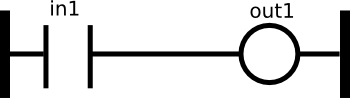
\includegraphics[width=\imgsmall]{./images/intro_fig1.png}
    \caption{Basic Ladder Logic Diagram}
    \label{fig:intro_fig1}
\end{figure}

The most basic structure of ladder logic is shown in figure \ref{fig:intro_fig1}. 
We have 
$$M=\lbrace in_1 \rbrace, S=\lbrace out_1 \rbrace, C=\lbrace out_1 \rbrace, R=\lbrace rung_1 \rbrace, P=\lbrace L,R \rbrace.$$
Note that $rung_1$ is not explicitly labeled in ladder logic but we give it a name here
so we may demonstrate our language framework.

The symantics of figure \ref{fig:intro_fig1} is then: 
\begin{table}[htp]
    \centering
    \begin{tabular}{|l|l|l|}
        \hline
        Action & Result \\
        \hline
        $@T(in_1 = true)$ & $out_1 := true$ \\
        \hline
        $@T(in_1 = false)$ & $out_1 := false$ \\
        \hline
    \end{tabular}
    \caption{Semantics for Fig \ref{fig:intro_fig1}}
    \label{table:table_for_fig1}
\end{table}


Where $@T(<condition>)$ is used to denote the positive edge of a condition becoming true.
We also assume negligable delay between the action occuring and the result being asserted.
It is important to note that our function table must be complete that is have an entry for
all possible combinations in the input domain.

\begin{figure}[htp]
    \centering
    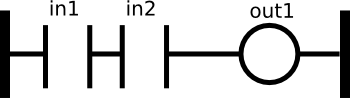
\includegraphics[width=\imgsmall]{./images/intro_fig2.png}
    \caption{Simple AND Logic Diagram}
    \label{fig:intro_fig2}
\end{figure}

When multiple actions are connected on the same rung it is interpreted as a logical AND 
expression. In figure \ref{fig:intro_fig2} we can expand our model to:

$$M=\lbrace in_1, in_2 \rbrace, S=\lbrace out_1 \rbrace, C=\lbrace out_1 \rbrace, R=\lbrace rung_1 \rbrace, P=\lbrace L,R \rbrace.$$

We can see that both $in_1$ and $in_2$ are on $rung_1$. This is interpreted as follows:

\begin{table}[htp]
    \centering
       \begin{tabular}{|l|l|l|}
        \hline
        Action & Result \\
        \hline
        $@T(in_1 = true \wedge in_2 = true)$ & $out_1 := true$ \\
        \hline
        $@T(in_1 = false \vee in_2 = false)$ & $out_1 := false$ \\
        \hline
    \end{tabular}
    \caption{Semantics for Fig \ref{fig:intro_fig2}}
    \label{table:table_for_fig2}
\end{table}

The conditions $in_1$ and $in_2$ are combined to form our composed action $@T(in_1 = true \wedge in_2 = true)$ 
as seen in table \ref{table:table_for_fig2}. We also note that there is no action for each individual condition
becoming true nor do we need to individually calculate the timing on $in_1$ or $in_2$ individually.

\begin{figure}[htp]
    \centering
    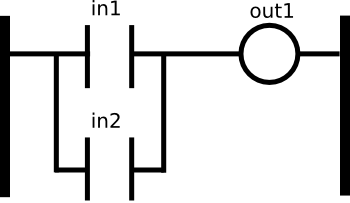
\includegraphics[width=\imgsmall]{./images/intro_fig3.png}
    \caption{Branching Rungs}
    \label{fig:intro_fig3}
\end{figure}


In addition to mutiple actions connected to the same rung, actions can also be branched. A branched rung as
show in figure \ref{fig:intro_fig3} behaves like a logical OR. In addition two or more rungs can be joined
as show in figure \ref{fig:intro_fig3a}. The semantics are equivalent in both figure \ref{fig:intro_fig3} and 
figure \ref{fig:intro_fig3a}.

\begin{figure}[htp]
    \centering
    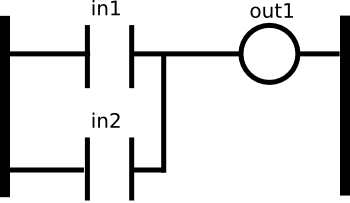
\includegraphics[width=\imgsmall]{./images/intro_fig3a.png}
    \caption{Branching Rungs (Alternative)}
    \label{fig:intro_fig3a}
\end{figure}

\begin{table}[htp]
    \centering
       \begin{tabular}{|l|l|l|}
        \hline
        Action & Result \\
        \hline
        $@T(in_1 = true \vee in_2 = true)$ & $out_1 := true$ \\
        \hline
        $@T(in_1 = false \wedge in_2 = false)$ & $out_1 := false$\\
        \hline
    \end{tabular}
    \caption{Semantics for Fig \ref{fig:intro_fig3} and Fig \ref{fig:intro_fig3a}}
    \label{table:table_for_fig3}
\end{table}

Since the semantics are the same for both figure \ref{fig:intro_fig3} and figure \ref{fig:intro_fig3a} we can
express both outcomes with function table \ref{table:table_for_fig3}.
As before in table \ref{table:table_for_fig2} in table \ref{table:table_for_fig3} $in_1$ and $in_2$ are composed to form our composed action $@T(in_1 = true \vee in_2 = true)$. However it is also possible to represent this action another way.

\begin{table}[htp]
    \centering
       \begin{tabular}{|l|l|l|}
        \hline
        Action & Result \\
        \hline
        $@T(in_1 = true)$ & $out_1 := true$ \\
        \hline
        $@T(in_2 = true)$ & $out_1 := true$ \\
        \hline
        $@T(in_1 = false \wedge in_2 = false)$ & $out_1 := false$\\
        \hline
    \end{tabular}
    \caption{Semantics for Fig \ref{fig:intro_fig3} and Fig \ref{fig:intro_fig3a}}
    \label{table:table_for_fig3a}
\end{table}

In table \ref{table:table_for_fig3a} we choose to represent $in_1$ and $in_2$ as seperate actions. This matches figure
\ref{fig:intro_fig3a} more closely but also makes any verification harder than table \ref{table:table_for_fig3}. For
smaller examples table \ref{table:table_for_fig3} make more sense since you can verify relatively simple smaller functions
quite fast. If a system becomes resonably large however there might be motivation to use the style shown in 
table \ref{table:table_for_fig3a} since it will allow more complex functions to be decomposed into simpler actions.
Since semantically the two are equivalent this paper will focus to the first convention.




%not sure if I should put rung definition here
\pagebreak[4]

\begin{figure}[htp]
    \centering
    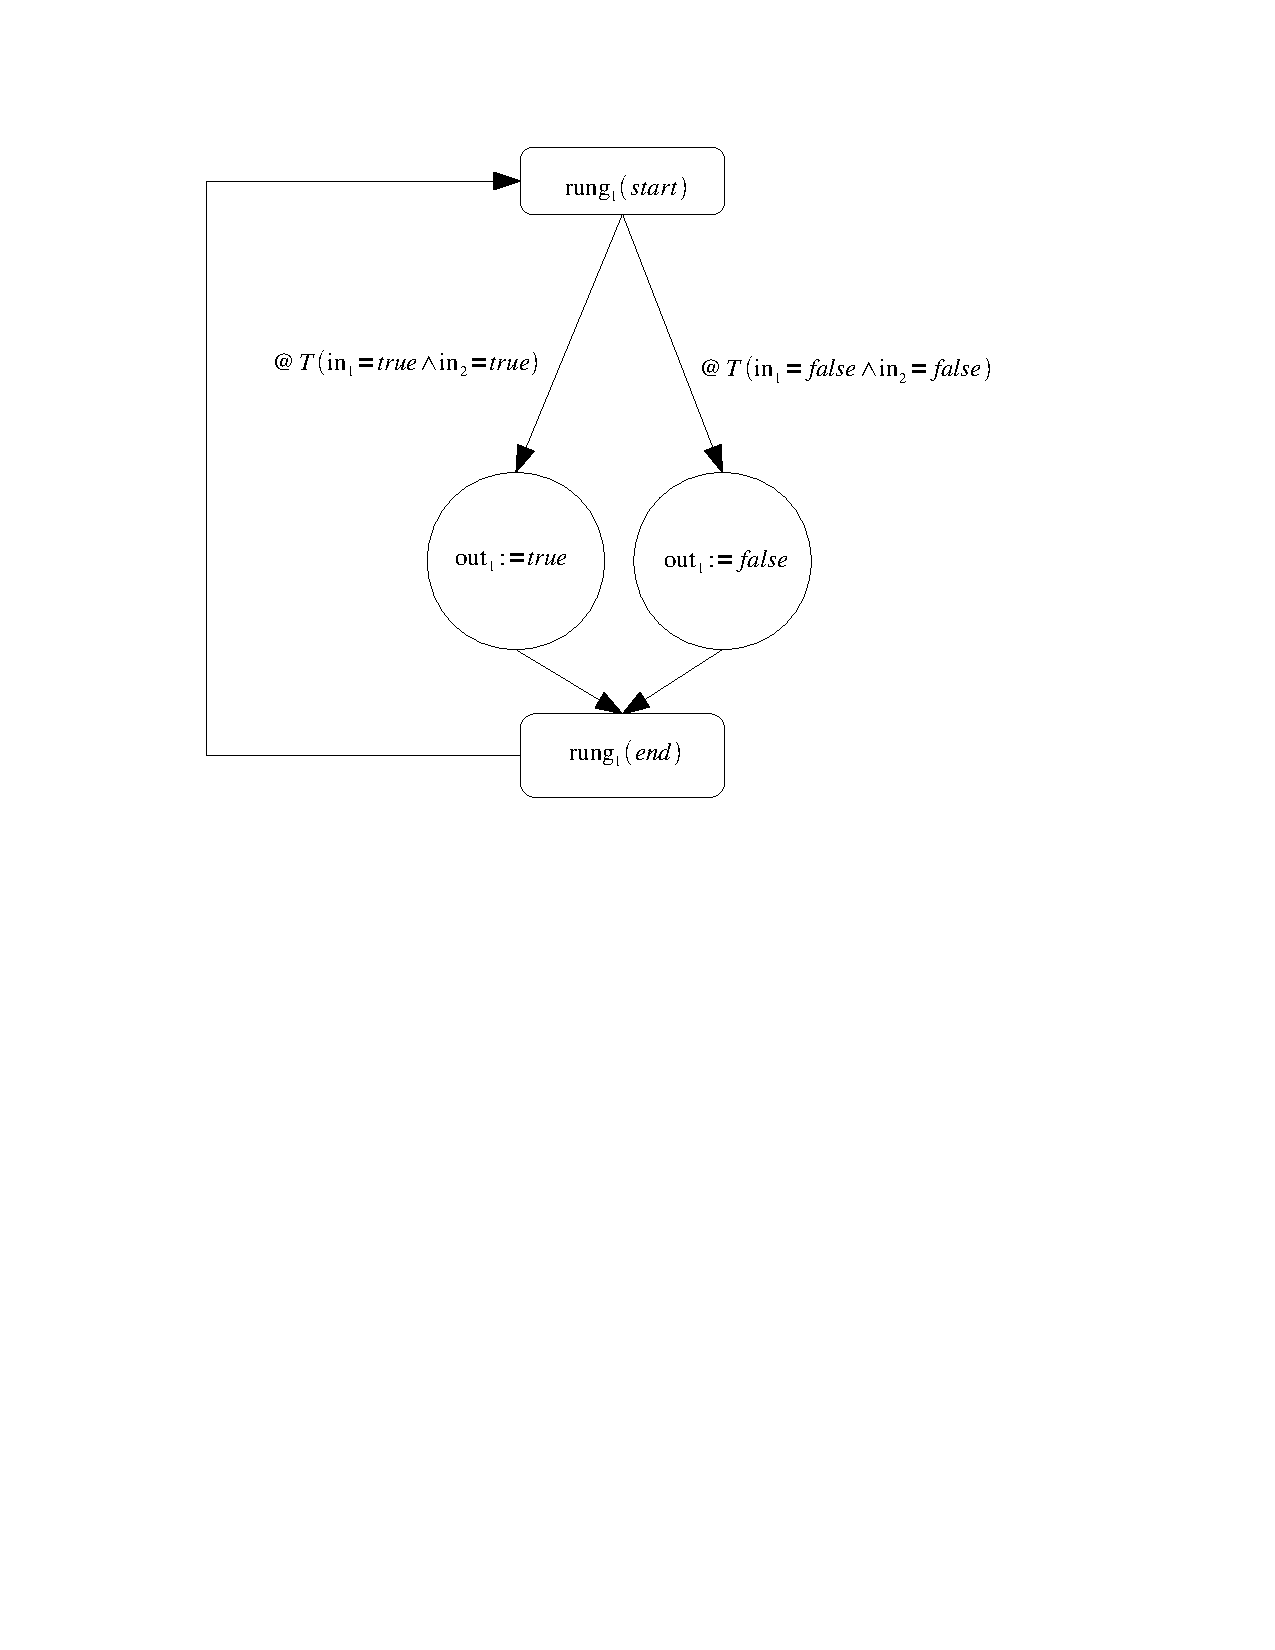
\includegraphics[trim= 50mm 140mm 50mm 10mm, clip ,width=\imgmedsmall]{./images/intro_and_graph.pdf} %custom size
    \caption{State chart conversion for table \ref{table:table_for_fig2}}
    \label{fig:intro_and_graph}
\end{figure}

A rung can be defined as a directed acyclic graph with exactly one source and one sink. The state variables form guard conditions along the edges. A branch in this case represents 2 edges leaving one node. For example figure \ref{fig:intro_fig2}
can be easily converted into a state chart by observing the results in table \ref{table:table_for_fig2}. 
Each row of table \ref{table:table_for_fig2} is directly converted into an edge with the appropriate guard conditions.
Each output assertion is given their own state. Finally in figure \ref{fig:intro_and_graph} we observe 1 source for the
graph being the start state of the rung, and one sink for the graph being the end state for the rung. We can equivalently take figure \ref{fig:intro_fig3} observe its function table \ref{table:table_for_fig3} and produce an equivalent state chart from its function table.

\pagebreak[3]

\begin{figure}[htp]
    \centering
    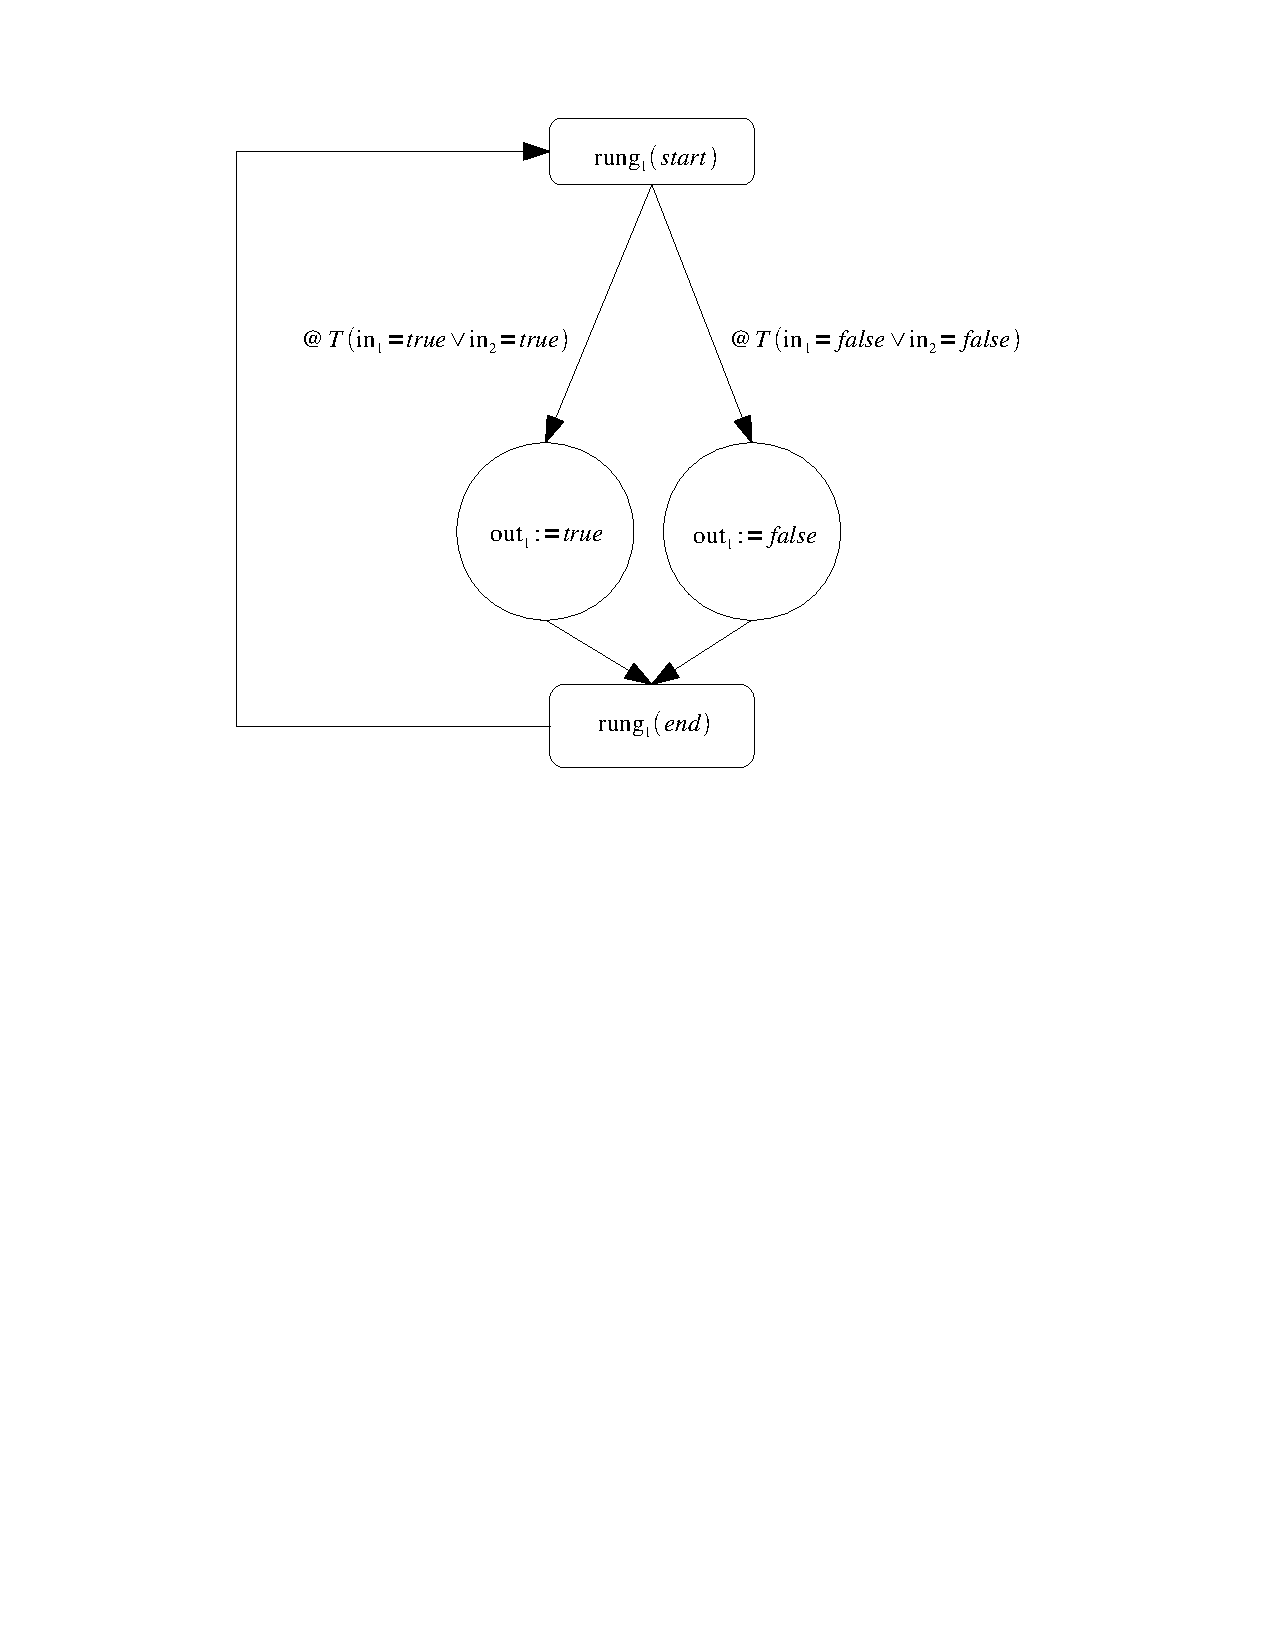
\includegraphics[trim= 50mm 140mm 50mm 10mm, clip ,width=\imgmedsmall]{./images/intro_or_graph.pdf} %custom size
    \caption{State chart conversion for table \ref{table:table_for_fig3}}
    \label{fig:intro_or_graph}
\end{figure}

Thus, each rung can be converted into an equivalent state chart by examining its 
function table, assigning the state variables to guard conditions, and creating a
state for each of the outputs. For completeness we complete this procedure to produce
a state chart equivalent representation for figure \ref{fig:intro_fig3a} and its
corresponding table \ref{table:table_for_fig3a}.


\begin{figure}[htp]
    \centering
    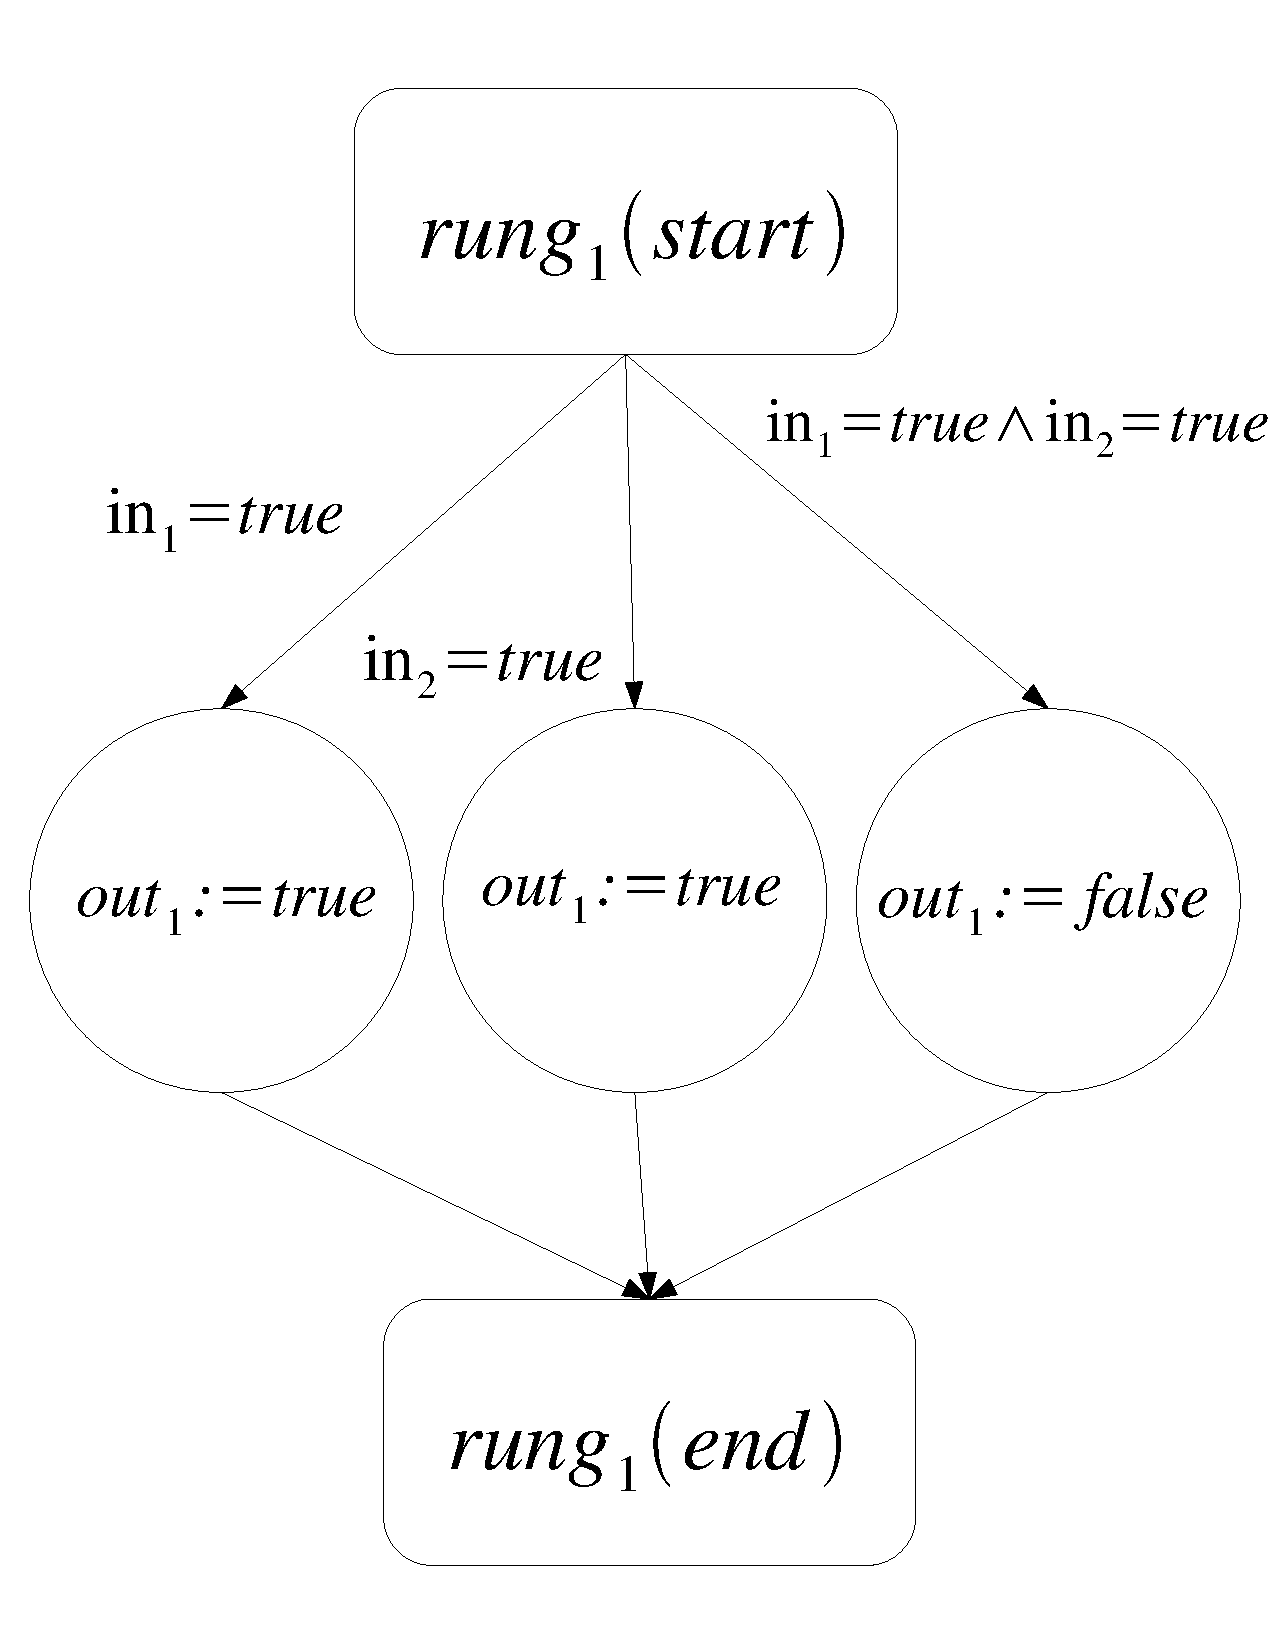
\includegraphics[width=\imgmedsmall]{./images/intro_or_graph_3a.pdf} %custom size
    \caption{State chart conversion for table \ref{table:table_for_fig3a}}
    \label{fig:intro_or_graph_3a}
\end{figure}

So far we've been looking at logic that has things happening instantaneously however ladder logic does contain methods for expressing more advance behavior. Suppose you have a light that you want to be able to turn on and stay on after you push a button. With any of the ladder diagrams shown above the light would go out as soon as the buttons were all released. In order to keep the light on and constantly on after the button is pressed we introduce the concept of a latch. We modify our diagram shown in figure \ref{fig:intro_fig3a} making the output feed back into one of the inputs to our OR circuit. The result is show in figure \ref{fig:intro_fig_latched}.

%figure for latched circuits 
\begin{figure}[htp]
    \centering
    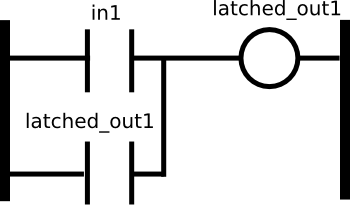
\includegraphics[width=\imgsmall]{./images/intro_fig_latched.png} 
    \caption{Latched ladder logic circuit.}
    \label{fig:intro_fig_latched}
\end{figure}

The latched circuit operates the same way as the behavior show in \ref{table:table_for_fig3a} the key difference is the feedback of the OR circuit replaces the second row of the function table.
